    \documentclass[conference]{IEEEtran}
%\usepackage[spanish]{babel} % Obligatorio para papers en Español de JAR 2017
%\usepackage[spanish,es-tabla]{babel} % Cambia Cuadro por Tabla (OK en Linux & Overleaf)

\usepackage[spanish,es-tabla]{babel} % para acentos en español
\usepackage[utf8]{inputenc} % para poder copiar acentos desde el pdf
\usepackage[T1]{fontenc} % para poder copiar acentos desde el pdf

\usepackage{cite}
\usepackage{amsmath,amssymb,amsfonts}
\usepackage{algorithmic}
\usepackage{graphicx}
\usepackage{textcomp}
\usepackage{graphicx}
\usepackage[hidelinks]{hyperref} % to use \href{} command
\usepackage[caption=false]{subfig}
\usepackage{xcolor}
\usepackage{graphics} % for pdf, bitmapped graphics files
\usepackage{epsfig} % for postscript graphics files
\usepackage{color}
\usepackage{booktabs} % \toprule \midrule
\usepackage{threeparttable}
\usepackage[per-mode=symbol]{siunitx} % to handle units
\usepackage{tabularx} % INTENTAR REMOVERLO
\usepackage{comment}


\def\BibTeX{{\rm B\kern-.05em{\sc i\kern-.025em b}\kern-.08em
    T\kern-.1667em\lower.7ex\hbox{E}\kern-.125emX}}

\newcommand{\furl}[1]{\footnote{\url{#1}}}


\DeclareSIUnit\px{px} % declare pixel unit
\sisetup{separate-uncertainty} % for uncertainty number in siunitx

\usepackage{amsmath}
\usepackage{amssymb}
\usepackage{amsopn}
\usepackage{mathtools}

% math
\renewcommand{\vec}[1]{\boldsymbol{\mathbf{#1}}}
\newcommand{\norm}[1]{\left\lVert#1\right\rVert}

% Declare arg max and arg min functionss
\DeclareMathOperator*{\argmax}{arg\,max}
\DeclareMathOperator*{\argmin}{arg\,min}

% Homogeneous decoration function
\newcommand{\homo}[1]{\dot{#1}}


% Declare projection as math function
% Reescribir los operadores en los que se requiera usar juntos fromCoord y toCoord (no borrar fromCoord ni toCoord)
\DeclareMathOperator{\proj}{proj}
\newcommand{\fromCoord}[2]{{#1}_\mathrm{#2}}
\newcommand{\toCoord}[2]{{#1}^\mathrm{#2}}
\newcommand{\worldCoordSystem}{\mathit{W}}
\newcommand{\bodyCoordSystem}{\mathit{B}}
\newcommand{\firstGPSCoordSystem}{\mathit{G}}
\newcommand{\cameraCoordSystem}{\mathrm{c}}
\newcommand{\coordIndex}[2]{{#1}_{#2}}
\newcommand{\point}{\vec{p}}
%\newcommand{\worldPoint}{\toCoord{\point}{\worldCoordSystem}}
%\newcommand{\imagePoint}{\vec{u}}
%\newcommand{\cameraPoint}{\toCoord{\point}{\cameraCoordSystem}}
%\newcommand{\homoWorldPoint}{\toCoord{\homo{\point}}{\worldCoordSystem}}
%\newcommand{\homoImagePoint}{\homo{\imagePoint}}
%\newcommand{\homoCameraPoint}{\toCoord{\homo{\point}}{\cameraCoordSystem}}
\newcommand{\measurement}{\vec{z}}
\newcommand{\noisyMeasurement}{\hat{\vec{z}}}
%\newcommand{\seMatrix}{\vec{\xi}}
%\newcommand{\transform}[2]{\toCoord{\fromCoord{\seMatrix}{#2}}{#1}}
\newcommand{\pointCoord}[1]{\toCoord{\point}{#1}}
\newcommand{\rotation}{\vec{R}}
\newcommand{\rotationCoord}[2]{\rotation_{#2}^{#1}}
\newcommand{\translation}{\vec{t}}
\newcommand{\translationCoord}[2]{\translation_{#2}^{#1}}
\newcommand{\rigidTransform}{\vec{T}}
\newcommand{\rigidTransformCoord}[2]{\rigidTransform_{#2}^{#1}}
\newcommand{\intrinsicMatrix}{\vec{K}}
\newcommand{\principalPoint}{\vec{c}}
\newcommand{\reprojectionError}{u}
\newcommand{\projectionMatrix}{\vec{P}}
\newcommand{\cameraCenter}{\vec{o}}
\newcommand{\worldCameraCenter}{\toCoord{\cameraCenter}{\worldCoordSystem}}
\newcommand{\essentialMatrix}{\vec{E}}
\newcommand{\fundamentalMatrix}{\vec{F}}
\newcommand{\inverse}[1]{{#1}^{-1}}
\newcommand{\identityMatrix}{\vec{I}}

% Motion model
\newcommand{\position}{\vec{p}}
\newcommand{\orientationQuaternion}{\vec{q}}
\newcommand{\predictedPosition}{\hat{\vec{p}}}
\newcommand{\predictedOrientationQuaternion}{\hat{\vec{q}}}
\newcommand{\linearVelocity}{\vec{v}}
\newcommand{\angularVelocity}{\vec{\omega}}

\DeclareMathOperator{\slerpOp}{slerp}
\newcommand{\slerp}[1]{\slerpOp{\left( #1 \right)}}

\newcommand{\residual}{\vec{e}}
\newcommand{\weightMatrix}{\vec{W}}
\newcommand{\covMatrix}{\vec{\Sigma}}
\newcommand{\systemState}{\vec{x}}
\newcommand{\bias}{\vec{b}}
%\newcommand{\biasAcc}{\coordIndex{\bias}{a}}
%\newcommand{\biasGyro}{\coordIndex{\bias}{g}}

% Map structure
\newcommand{\map}{M}
\newcommand{\keyframesSet}{K}
\newcommand{\mapPointsSet}{P}
\newcommand{\observedMapPoints}{O}
\newcommand{\covisibilityKeyframes}{CK}
\newcommand{\localMap}{local\_map}



% Bundle Adjutment
\newcommand{\update}{\vec{\delta}}
\newcommand{\incremental}{\hat{\update}}


% Loop Closure names

% scaled operators and letters to fancy view
\newcommand{\sminus}{\scalebox{0.5}[1.0]{$-$}}
\newcommand{\splus}{\scalebox{0.6}[0.6]{$+$}}
\newcommand{\curr}{c}
\newcommand{\sind}[1]{\scalebox{0.6}[0.6]{$#1$}}
\newcommand{\ind}[1]{\scalebox{0.7}[0.7]{$#1$}}

\newcommand{\keyframe}{\vec{K}}
\newcommand{\bowVector}{\vec{v}}
\newcommand{\lcError}{\vec{\Omega}}
\newcommand{\relativeTransformation}{\seMatrix}
\DeclareMathOperator{\interpolate}{interpolate}

\newcommand{\relativeMotion}{\vec{\delta}}
\newcommand{\groundTruth}[1]{{#1}^{*}}



% definición del operador rot()
\DeclareMathOperator{\rotationOp}{rot}
\newcommand{\getRotation}[1]{\rotationOp{\left( #1 \right)}}

\DeclareMathOperator{\translationOp}{trans}
\newcommand{\getTranslation}[1]{\translationOp{\left( #1 \right)}}









\begin{document}
%
% paper title
% Titles are generally capitalized except for words such as a, an, and, as,
% at, but, by, for, in, nor, of, on, or, the, to and up, which are usually
% not capitalized unless they are the first or last word of the title.
% Linebreaks \\ can be used within to get better formatting as desired.
% Do not put math or special symbols in the title.
%\title{Fusión de sensores de robot desmalezador en entorno simulado}
%\title{Lightweight VI-SLAM with Asynchronous Loop Closure and Square Root Global Bundle Adjustment}
\title{VI-SLAM Eficiente con Cierre de Ciclos Asíncrono y Bundle Adjustment Global por Factorización QR}

%\author{\IEEEauthorblockN{1\textsuperscript{st} Tomás Santucci}
%\IEEEauthorblockA{\textit{Departamento de Ciencias de la Computación} \\
%\textit{FCEIA-UNR}\\
%Rosario, Argentina\\
%tomassantucci0@gmail.com}
%\and
%\IEEEauthorblockN{2\textsuperscript{nd} Mateo De Mayo}
%\IEEEauthorblockA{
%\textit{Technical University of Munich}\\
%Munich, Alemania\\
%mateo.demayo@tum.de}
%\and
%\IEEEauthorblockN{3\textsuperscript{rd} Taihú Pire}
%\IEEEauthorblockA{\textit{CIFASIS} \\
%\textit{CONICET-UNR}\\
%Rosario, Argentina \\
%pire@cifasis-conicet.gov.ar}
%\and
%\IEEEauthorblockN{2\textsuperscript{nd} Daniel Cremers}
%\IEEEauthorblockA{
%\textit{Technical University of Munich}\\
%Munich, Alemania\\
%cremers@tum.de}
%}

\author{%
\IEEEauthorblockN{Tomás Santucci\textsuperscript{1},
Mateo De Mayo\textsuperscript{2},
Taihú Pire\textsuperscript{3},
Daniel Cremers\textsuperscript{2}}
\IEEEauthorblockA{\textsuperscript{1}\textit{Departamento de Ciencias de la Computación, FCEIA-UNR}, Rosario, Argentina \\
\textsuperscript{2}\textit{Technical University of Munich}, Munich, Alemania \quad
\textsuperscript{3}\textit{CIFASIS, CONICET-UNR}, Rosario, Argentina \\
tomassantucci0@gmail.com \quad \{mateo.demayo, cremers\}@tum.de \quad pire@cifasis-conicet.gov.ar}
}

%\author{\vspace{5\baselineskip}}

% make the title area
\maketitle

% As a general rule, do not put math, special symbols or citations
% in the abstract
\begin{abstract}
% \todo[inline]{cada oración dice algo importante}
% \todo[inline]{oración de contexto: importancia de VI en XR}

%En aplicaciones de realidad extendida (XR) es indispensable que el sistema de localización del dispositivo sea robusto frente a movimientos bruscos y oclusiones en las cámaras. A su vez para que la experiencia de usuario sea fluida e inmersiva debe ser liviano para que pueda correr en tiempo real. Los dispositos XR, como los cascos de realidad virtual (VR), combinan múltiples cámaras e IMU que pueden ser usados por métodos de Odometría Visual-Inercial (VIO) para estimar su localización. 

% \todo[inline]{una o dos oraciones que describan el método brevemente}
%En este paper se propone un sistema VIO capaz de estimar la localización de dispositivos XR. El sistema propuesto tiene como punto de partida al algoritmo de Basalt, con lo cual mantiene una ventana de keyframes que optimiza y marginaliza de forma inteligente para mantener el sistema computacionalmente eficiente, y la vez lo extiende permitiendo trabajar con cascos con más de dos cámaras no paralelas, utiliza la IMU para predecir la localización y es capaz de reidentificar features perdidas por oclusiones o movimientos bruscos.
%\todo[inline]{BRUNO: Agregar comentario recall} 
% Keyframes y landmarks son almacenados en un mapa persistente que es utilizado luego para reconocer lugares previamente visitados. 

%\todo[inline]{COMPLETAR: Una oración de experimentos y resultados.}
%Se realizaron experimentos sobre un dataset de un casco de XR para validar el sistema VIO desarrollado. Los resultados muestran que el sistema logra una mayor robustez y precisión, y una trayectoria suave, requerimientos necesarios para aplicaciones XR.

% also add smart map management
%We present an efficient visual-inertial SLAM system that extends the Basalt visual-inertial odometry framework with persistent map management, real-time loop closure and large-scale optimization capabilities. Our approach integrates a lightweight loop closure module inspired by keyframe-based visual SLAM methods with the Basalt VIO front-end, enabling global consistency without sacrificing real-time performance. For global optimization, we adapt the RootBA formulation to support stereo and fisheye camera models with arbitrary calibration, providing numerically stable and hardware-friendly bundle adjustment suitable for large-scale maps. The resulting system combines the robustness and drift resistance of Basalt's visual-inertial front-end with the efficiency of square root bundle adjustment, achieving superior trajectory consistency and scalability. We evaluate on the EuRoC, TUM-VI, and Monado datasets, where our method achieves state-of-the-art absolute trajectory error in the indoor sequences and real-time performance, superior to other alternatives.

%Los sistemas de localización y mapeo visual-inercial deben operar en tiempo real sobre
%plataformas con recursos computacionales y energéticos estrictamente acotados, sin
%comprometer la precisión ni la robustez ante condiciones desafiantes.
%Los sistemas VIO del estado del arte logran performance en tiempo real pero acumulan \textit{drift} sin posibilidad de corrección global; los sistemas VI-SLAM existentes, por su parte,
%presentan dificultades para garantizar operación en tiempo real en escenarios típicos de
%robótica y VR/AR.
%En este trabajo presentamos un sistema de VI-SLAM eficiente que
%extiende el algoritmo de VIO Basalt con gestión de mapa
%persistente, detección y cierre de ciclos en tiempo real, y optimización a gran escala.
%El sistema incorpora un módulo de \textit{loop closure} liviano basado en HashBoW con
%arquitectura asíncrona, que permite la corrección global del \textit{drift} sin degradar
%la performance del front-end. Para la optimización global, adaptamos la formulación de
%RootBA para soportar sistemas multicámara con modelos de cámara arbitrarios, proveyendo un bundle adjustment numéricamente estable y
%ejecutable con precisión simple.
%Evaluamos el sistema en los datasets EuRoC, TUM-VI y
%Monado, donde el método propuesto alcanza un error de trayectoria absoluta
%del estado del arte en secuencias de interior, mantiene operación en
%tiempo real incluso en trayectorias de extensa duración, y demuestra robustez en
%condiciones desafiantes como escenas con baja textura gracias al front-end de Basalt.


Los sistemas VI-SLAM deben operar en tiempo real sobre plataformas con recursos
computacionales y energéticos estrictamente acotados, sin comprometer precisión ni
robustez. Los sistemas VIO del estado del arte logran rendimiento en tiempo real pero
acumulan \textit{drift} sin posibilidad de corrección global; los sistemas VI-SLAM
existentes, por su parte, presentan dificultades para garantizar operación en tiempo
real en escenarios típicos de robótica y realidad virtual/aumentada (VR/AR). En este trabajo presentamos un sistema VI-SLAM eficiente que extiende el algoritmo de VIO de Basalt con mapa persistente, detección y cierre de ciclos en tiempo real, y optimización a gran escala. El sistema
incorpora un módulo de \textit{loop closure} liviano basado en HashBoW con arquitectura
asíncrona, que corrige el \textit{drift} global sin degradar el rendimiento del
front-end, y adapta la formulación de RootBA para soportar sistemas multicámara con
modelos de cámara arbitrarios, proveyendo un bundle adjustment numéricamente estable y
ejecutable con precisión simple. Evaluamos este sistema en los datasets EuRoC, TUM-VI y Monado,
donde el método alcanza un error de trayectoria absoluta del estado del arte en secuencias
de interior, mantiene operación en tiempo real en trayectorias de extensa duración, y
demuestra robustez en condiciones desafiantes gracias al front-end de Basalt.

\end{abstract}

\begin{IEEEkeywords}
SLAM Visual-Inercial, Loop Closure, Consistencia Global, Bundle Adjustment
\end{IEEEkeywords}

% For peerreview papers, this IEEEtran command inserts a page break and
% creates the second title. It will be ignored for other modes.
\IEEEpeerreviewmaketitle

\section{Introducción}
\label{sec:introduction}
\begin{figure}[tp]
    \centering
    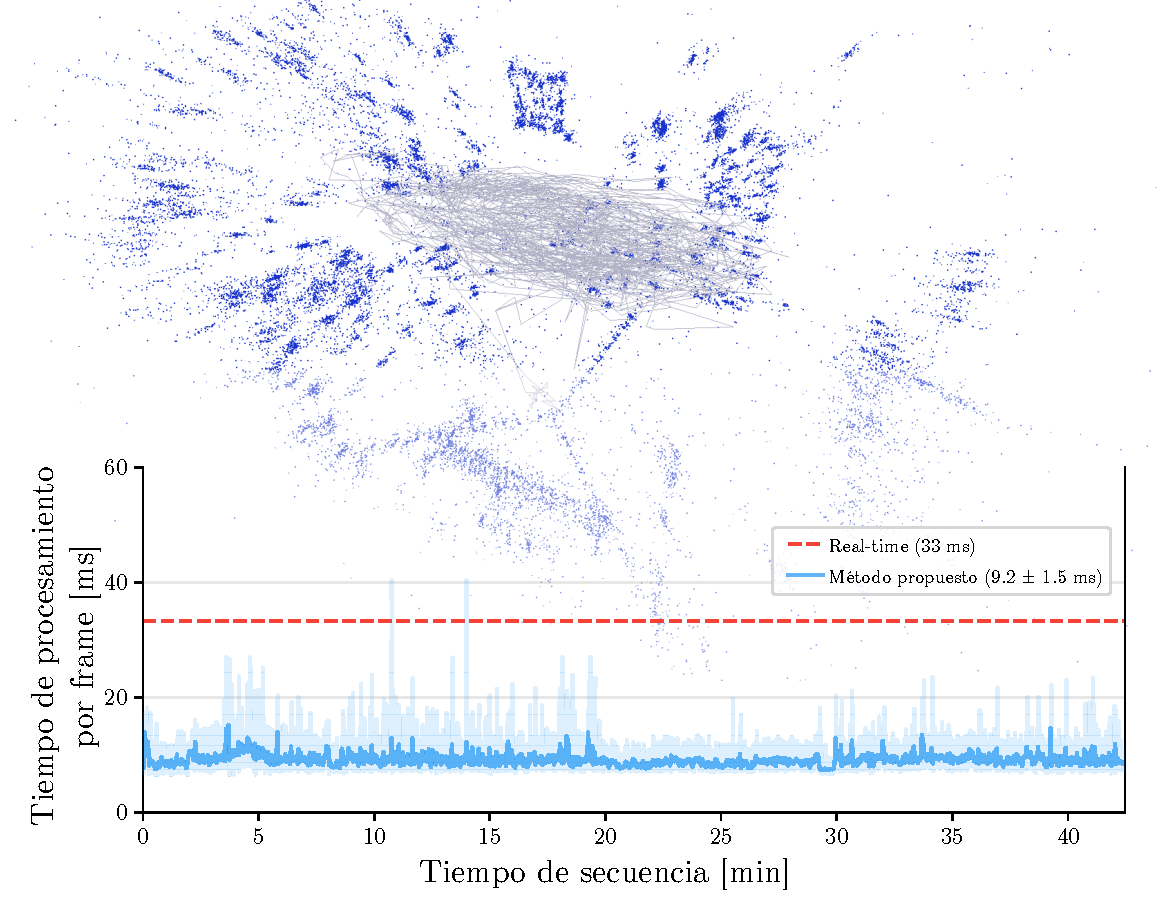
\includegraphics[width=1\linewidth]{images/abstract.mgo12.pdf}
    \caption{En la parte superior, un mapa de puntos generados por el sistema propuesto en la secuencia MGO12, de más de 40 minutos y cuatro cámaras, del Monado SLAM Dataset. En la parte inferior, una gráfica del tiempo de procesamiento por frame para esa secuencia. Se observa que el método opera por debajo del límite de tiempo real.}
    \label{fig:abstract-image}
\end{figure}

% PROBLEMA GENERAL
Los sistemas de robótica móvil y realidad virtual/aumentada (VR/AR) modernos operan frecuentemente
en plataformas con recursos computacionales y energéticos estrictamente acotados, como
nano drones (NAVs), robots móviles y headsets de VR/AR. Un sistema ineficiente no solo degrada la experiencia de usuario o el rendimiento del robot, sino que implica baterías más grandes, comprometiendo la viabilidad del sistema. Esto exige soluciones que operen en tiempo real sin depender de
hardware especializado como GPUs. Los métodos de SLAM geométricos son una alternativa
validada para entornos embebidos \cite{galagain2025semanticslamreadyembedded}. Sin embargo, cumplir
con los requisitos de tiempo real sigue siendo un desafío abierto: incluso sistemas VIO del
estado del arte presentan dificultades para garantizar robustez y procesamiento en tiempo real en
condiciones realistas \cite{demayo2025monadoslamdataset}. El desafío central es lograr precisión, eficiencia computacional y robustez, condiciones necesarias para ser desplegable en la práctica.

% VI-SLAM
La odometría visual-inercial (VIO) y el VI-SLAM fusionan cámaras
e IMU: la IMU provee estimaciones de alta frecuencia del movimiento mientras que las
cámaras aportan información rica del entorno, permitiendo estimaciones de pose precisas y
robustas ante condiciones desafiantes. El VI-SLAM además de estimar la localización, incorpora un mapa
persistente que habilita la detección de ciclos (loop closure) para corregir el drift acumulado y la reutilización del mapa, capacidades esenciales para una operación prolongada.

% OBJETIVO PRINCIPAL Y MÉTODO
El objetivo principal de este trabajo es desarrollar un sistema de VI-SLAM que aborde las limitaciones mencionadas. El método propuesto está basado en Basalt \cite{usenko2020basalt}, un sistema VIO del estado del arte para VR/AR, y es una extensión del trabajo \cite{zanotti2024basaltxr}, al que se le incorpora un mapa persistente y múltiples mejoras detalladas en la Sección \ref{sec:method}.

% CONTRIBUCIONES
El sistema propuesto extiende Basalt con un mapa persistente gestionado de manera inteligente, detección y cierre de ciclos con técnicas eficientes, y bundle adjustment adaptado de \textit{Structure from Motion} (SfM). Las principales contribuciones son:
\begin{itemize}
    \item Una extensión de Basalt con mapa persistente, cuya arquitectura basada en comunicación asíncrona entre componentes evita que las operaciones costosas del mapa degraden el rendimiento del sistema. Incorpora dos nuevos componentes que interactúan con el back-end de Basalt e implementan: detección de ciclos mediante HashBoW \cite{hashbow2024stricker} para recuperar eficientemente keyframes de contenido similar; optimización liviana del mapa mediante \textit{Pose Graph Optimization} para corregir el error acumulado luego de las detecciones de ciclos; fusión de mapa para asociar datos a largo plazo; y culling de keyframes para mantener el tamaño del mapa acotado, con heurísticas que priorizan keyframes de alta calidad visual y utilidad para la consistencia global.
    \item Un método eficiente y numéricamente estable de bundle adjustment para optimizar mapas resultantes de sistemas VI-SLAM multicámara con modelos de cámara arbitrarios. Se basa en RootBA \cite{demmelBasaltSquareRoot2021a}, que formula el problema mediante factorización QR, siguiendo la línea de \cite{demmelBasaltSquareRoot2021}, que lo aplicó por primera vez en la optimización local de Basalt.
    \item Una evaluación exhaustiva del sistema propuesto sobre datasets con amplia variedad de escenarios y desafíos típicos de robótica y VR/AR, en la que se mide rigurosamente la precisión y el rendimiento comparándolo con dos alternativas del estado del arte.
\end{itemize}

% CLAIMS
En resumen, el sistema alcanza una precisión comparable al estado del arte, principalmente en entornos típicos de VR/AR. También, es robusto ante condiciones desafiantes, como escenarios de baja textura, y mantiene la operación en tiempo real incluso en trayectorias de larga duración. Por último, el método de bundle adjustment propuesto es numéricamente estable y admite ejecución en precisión simple, lo que se traduce en una mejora de rendimiento considerable.


\section{Trabajo Relacionado}
\label{sec:related}
%\subsection{Visual SLAM}
%\label{subsec:visual_slam}

%Los fundamentos del SLAM moderno fueron establecidos por Davison et al. con
%\textbf{MonoSLAM}~\cite{davison2007monoslam}, el primer sistema monocular en
%tiempo real basado en EKF, y por Klein y Murray con
%\textbf{PTAM}~\cite{klein2007parallel}, que introdujo la separación entre
%seguimiento y mapeo en hilos paralelos, estableciendo el patrón arquitectónico
%de los sistemas posteriores basados en fotogramas clave.

%Engel et al. propusieron \textbf{LSD-SLAM}~\cite{engel2014lsd}, el primer
%sistema directo de gran escala, que opera sobre intensidades de píxeles en
%lugar de características extraídas explícitamente.
%Esta línea de métodos directos fue extendida por \textbf{SVO}~\cite{forster2014svo},
%que combina seguimiento directo con optimización del error de reproyección,
%por \textbf{DSO}~\cite{engel2018dso}, que formula la odometría directa
%sobre una ventana deslizante con calibración fotométrica conjunta, y por
%\textbf{DSM}~\cite{zubizarreta2020dsm}, que añade cierre de bucles al
%\emph{pipeline} directo.
%En paralelo, \textbf{ORB-SLAM2}~\cite{mur2017orbslam2} llevó los métodos
%basados en características a su madurez, incorporando cierre de bucles y
%relocalización robusta mediante vocabulario visual, convirtiéndose en la
%referencia principal de los sistemas indirectos.

A continuación se revisan los trabajos más relevantes en odometría y SLAM visual-inercial, organizados según el tipo de método empleado.

\subsection{Métodos basados en filtros}

Los primeros enfoques para odometría visual-inercial se apoyaron en la teoría de filtros de Kalman para estimar la pose del dispositivo.

MSCKF~\cite{mourikis2007msckf} propuso un algoritmo basado en un filtro de Kalman extendido (EKF) para sistemas VIO. Su contribución principal fue eliminar las posiciones 3D de los puntos del vector de estado, logrando una complejidad computacional lineal en el número de \textit{features} observados.
ROVIO~\cite{bloesch2015rovio} adoptó un enfoque alternativo mediante un filtro de Kalman extendido iterativo (IEKF), utilizando el error fotométrico sobre parches de imagen como medición.

\subsection{Métodos basados en optimización de mínimos cuadrados}

A diferencia de los métodos basados en filtros, la optimización de mínimos cuadrados en ventana deslizante demostró mayor precisión y eficiencia computacional. Tras consolidarse en sistemas de SLAM visual como PTAM~\cite{klein2007ptam} y ORB-SLAM~\cite{mur2015orbslam}, se estableció como el paradigma predominante en VI-SLAM.

OKVIS~\cite{leutenegger2015okvis} fue uno de los primeros sistemas en formular la fusión visual-inercial como un problema de mínimos cuadrados no lineales en ventana deslizante, acoplando errores de reproyección y preintegración de la IMU.
%VINS-Fusion~\cite{qin2019vinsfusion} es un sistema de VI-SLAM estéreo con loop closure mediante DBoW2, pose graph optimization y fusión de mapa. Su \textit{tracking} está basado en KLT e introduce soporte para múltiples sensores mediante una formulación generalizada de la optimización.
Basalt~\cite{usenko2020basalt} es un método de VIO basado en optimización de keyframes. En el \textit{front-end} emplea FAST~\cite{rosten2006fast} para la detección de features y \textit{optical flow} por KLT~\cite{lucas1981klt} para el tracking. El \textit{back-end} optimiza una ventana de keyframes con una heurística de marginalización que mantiene la eficiencia computacional: cada vez que un keyframe es removido, se calcula un término de marginalización que se incorpora en la siguiente optimización. Adicionalmente, los datos marginalizados por el VIO se procesan de manera \textit{offline} para construir un mapa global y recuperar nuevas correspondencias entre puntos, que son luego refinadas mediante bundle adjustment global sobre todas las poses y landmarks.
Kimera~\cite{rosinol2020kimera} es un sistema de \textit{metric-semantic} VI-SLAM que incorpora loop closure mediante DBoW2 y pose graph optimization. A diferencia de los sistemas tradicionales, integra además reconstrucción de malla y etiquetado semántico en 3D.
ORB-SLAM3~\cite{campos2021orbslam3} unificó múltiples modalidades de entrada con soporte para IMU, asociación de datos a corto, mediano y largo plazo, y un sistema de mapas Atlas para gestionar mapas desconectados. Se ha consolidado como uno de los sistemas VI-SLAM más precisos y ampliamente adoptados en la literatura.
OKVIS2~\cite{leutenegger2022okvis2} extiende OKVIS incorporando un mapa persistente con loop closure y marginalización eficientes, manteniéndose entre los sistemas de mayor precisión del estado del arte en benchmarks estándar como EuRoC~\cite{burri2016euroc} y TUM-VI~\cite{schubert2018tum}.
%\textbf{DM-VIO}~\cite{stumberg2022dmvio} adaptó el enfoque directo de DSO al entorno VI mediante marginalización retardada.
Snake-SLAM~\cite{ruckert2021snakeslam} propuso una optimización desacoplada que resuelve el estado de la IMU y el bundle adjustment visual como subproblemas independientes, reduciendo la complejidad computacional sin sacrificar precisión.
Basalt-XR~\cite{zanotti2024basaltxr} extiende Basalt al contexto de VR/AR, incorporando la posibilidad de asociar datos a mediano plazo mediante un mapa persistente que reintroduce keyframes en la ventana local del back-end.

En resumen, OKVIS2 y ORB-SLAM3 obtienen la mayor precisión del estado del arte~\cite{krishnan2025lamaria,leutenegger2022okvis2}, pero no logran ser robustos o cumplir los límites de tiempo real en entornos de VR/AR~\cite{demayo2025monadoslamdataset}. Basalt, en contraste, es un sistema de VIO robusto que alcanza métricas de precisión prometedoras y un rendimiento más eficiente, aun sin mapa persistente.

\subsection{Métodos basados en aprendizaje}
\label{subsec:learning_based}

Trabajos recientes han explorado el uso de redes neuronales en el \emph{pipeline} de SLAM, como DROID-SLAM~\cite{teed2021droid} y Deep Patch Visual SLAM~\cite{lipson2024dpvslam}, este último superador en velocidad frente a sus predecesores.
Si bien estos enfoques han alcanzado precisión del estado del arte, aún se encuentran en consolidación.
En contraste, el sistema propuesto en este trabajo es más ligero computacionalmente, no requiere entrenamiento supervisado y resulta más adecuado para plataformas con recursos restringidos.


\section{Método propuesto}
\label{sec:method}
\begin{figure}[!htbp]
    \centering
    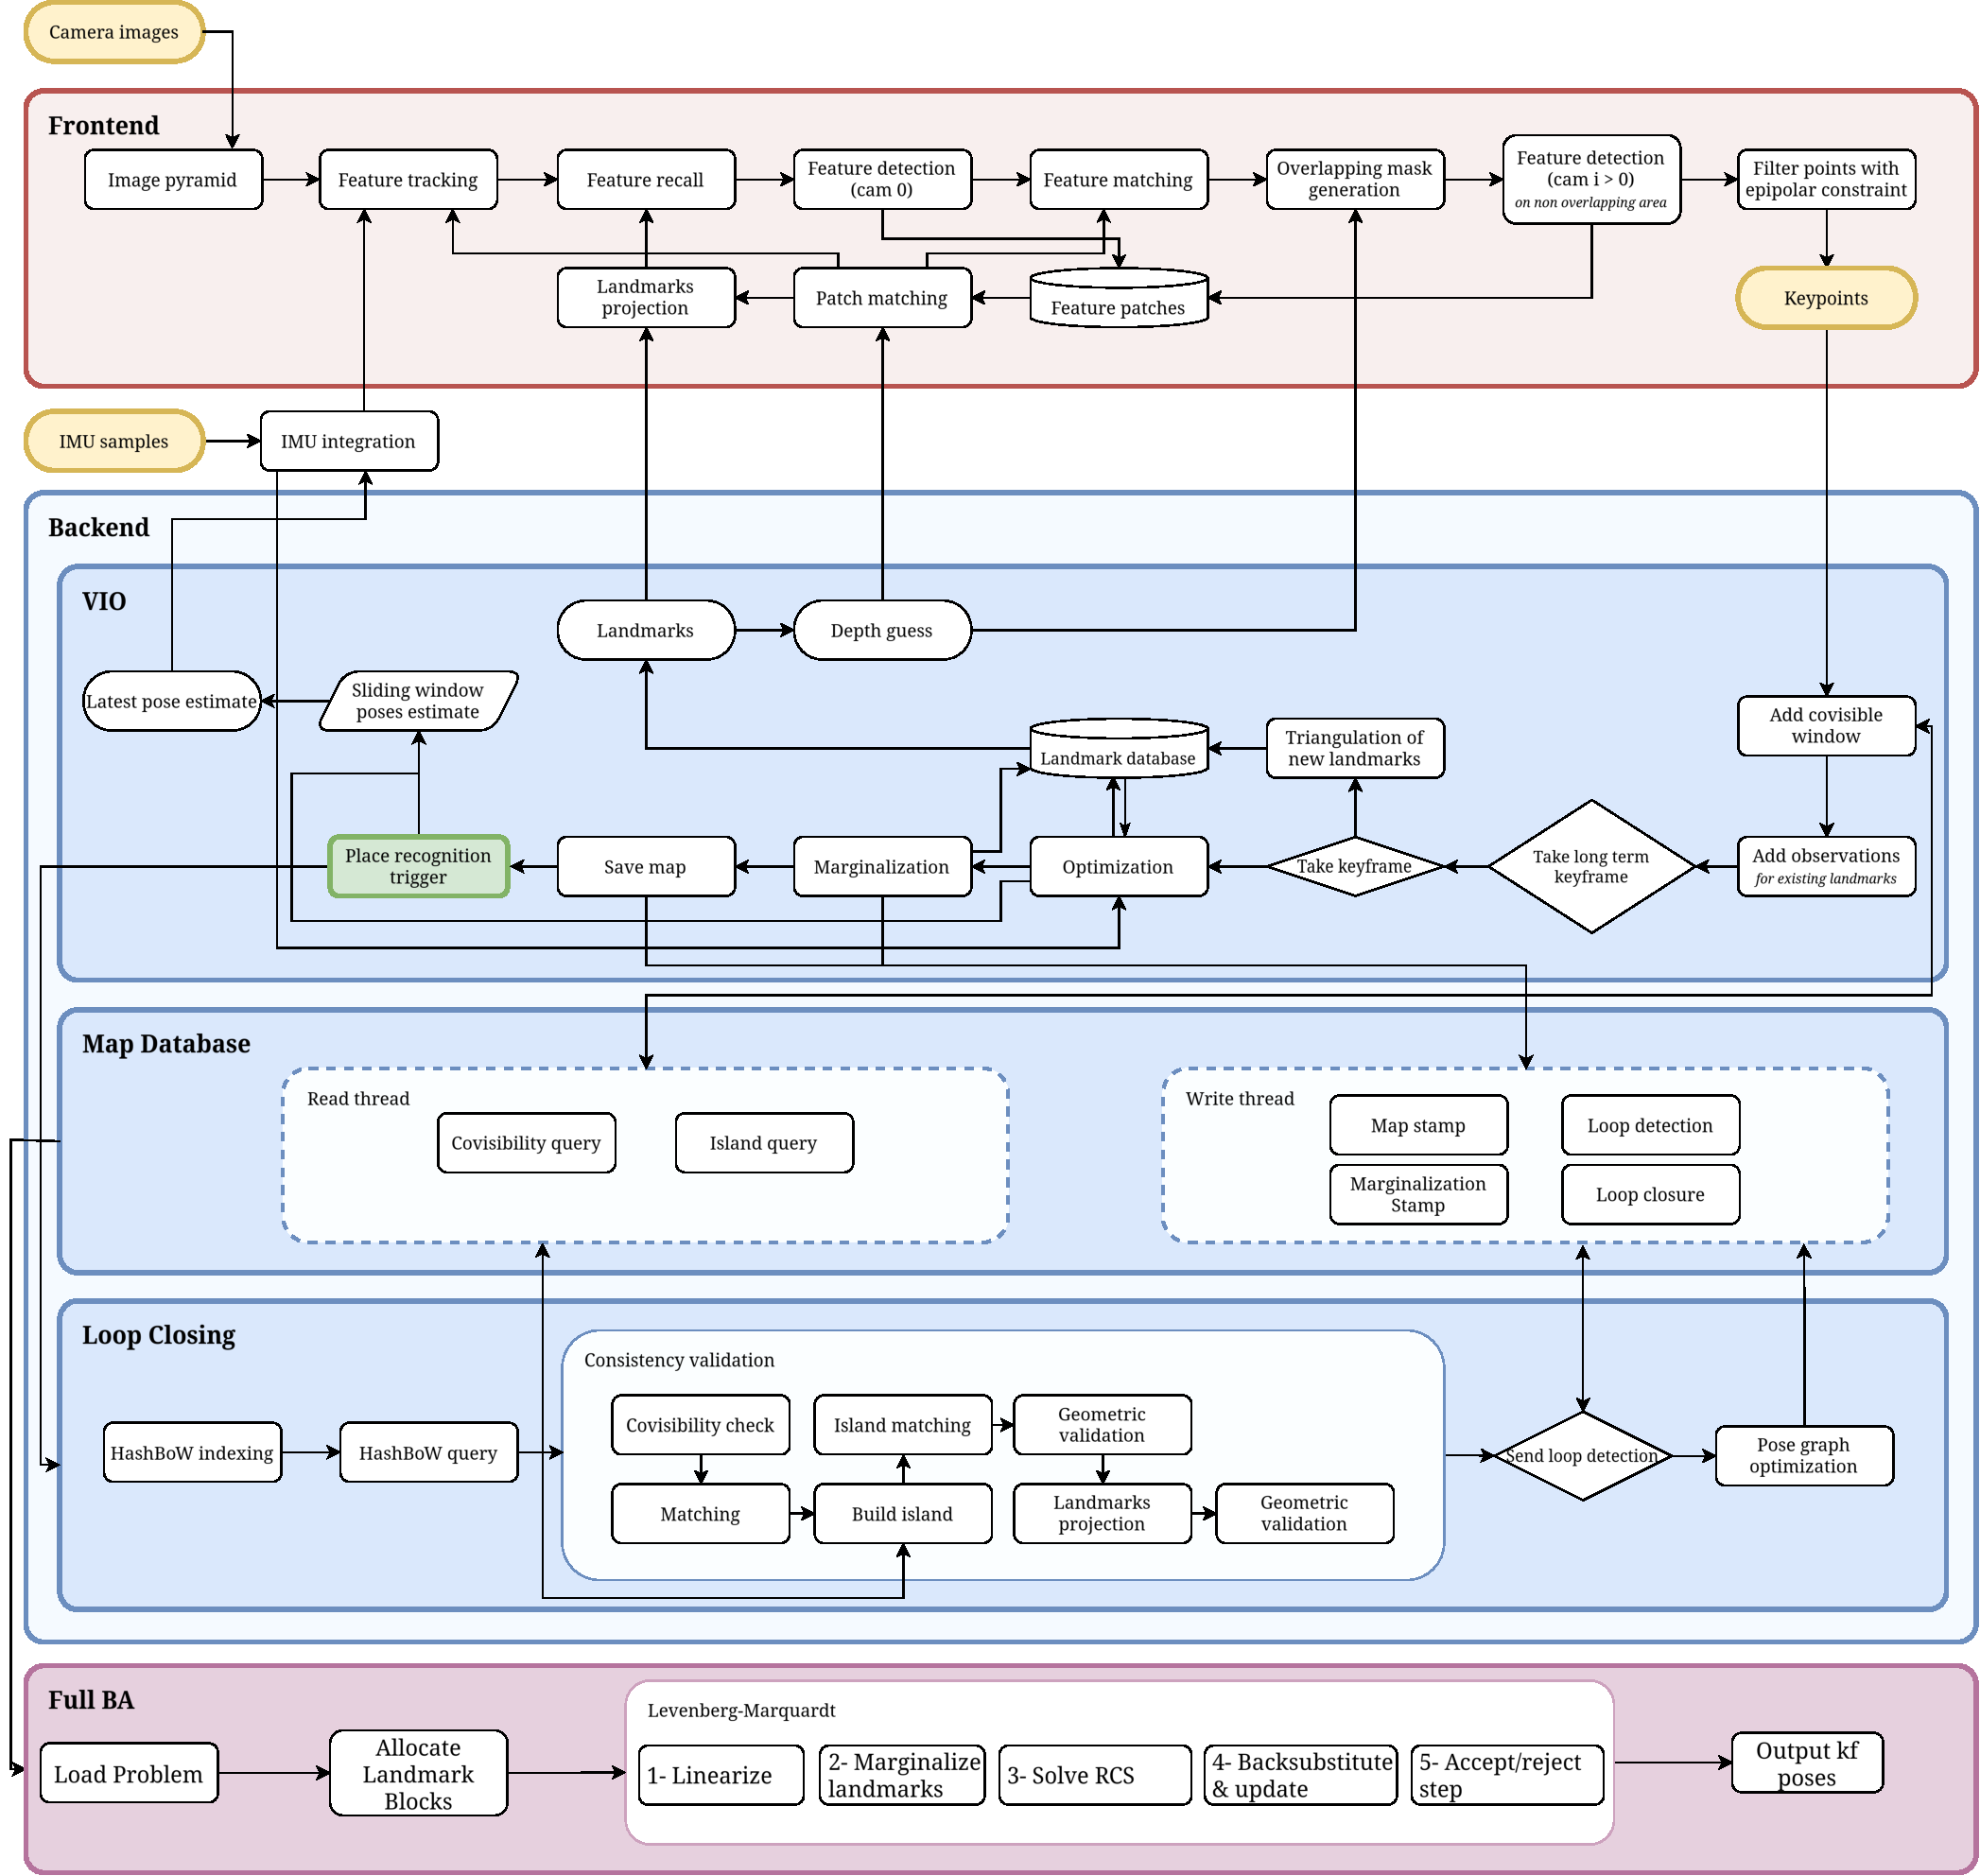
\includegraphics[width=1\linewidth]{images/system-arch.pdf}
    \caption{Arquitectura del sistema VI-SLAM propuesto. Se incorporan los componentes \texttt{Loop Closing} y \texttt{RootBA Full}, y se extiende \texttt{Map Database}.}
    \label{fig:system-pipeline}
\end{figure}

En este trabajo presentamos una serie de funcionalidades en Basalt (ver Figura \ref{fig:system-pipeline}), que lo transforman en un sistema VI-SLAM con precisión comparable al estado del arte. Tomamos como punto de partida BasaltXR \cite{zanotti2024basaltxr}, que a su vez extiende la versión de Basalt utilizada en \cite{demayo2025monadoslamdataset}.
Las mejoras están diseñadas para aumentar la precisión del sistema mediante el uso de información del mapa, manteniendo la eficiencia característica de Basalt.

\subsection{Mapa Persistente}

En primer lugar, se enriqueció la clase \texttt{MapDatabase} para soportar más operaciones y habilitar la utilización del mapa de manera más inteligente. Se implementó una estructura llamada \texttt{CovibilityGraph} que contiene grafos que acumulan información de interés y se mantienen actualizados en todo momento, inspirada en el \textit{Essential Graph}, introducido en \cite{campos2021orbslam3}. Entre ellos: un grafo pesado de covisibilidad, que se usa para resolver consultas del back-end y del componente de \texttt{LoopClosing} para la detección de ciclos; un árbol de expansión, que mantiene a todos los keyframes conectados y es utilizado al realizar Pose Graph Optimization; un grafo no dirigido que almacena aristas entre keyframes involucrados en cierres de ciclos; un grafo no dirigido, que guarda aristas que tengan un peso alto en el grafo de covisibilidad, y se utiliza en Pose Graph Optimization.

Además, se introdujo un mecanismo de culling de keyframes con dos estrategias, que evitan introducir keyframes redundantes al mapa, y que este crezca de manera indefinida: (1) Cada vez que el back-end marginaliza un keyframe, se verifica la redundancia de la información que aporta al mapa. Si más de un 90\% de sus observaciones corresponden a landmarks que ya son observados por, al menos, otros 3 keyframes del mapa, se elimina. (2) Cada vez que el mapa supera un total de 1500 keyframes, se eliminan 30 de ellos. Para seleccionarlos, se utiliza una suma pesada de diferentes heurísticas como función de scoring. Este puntaje penaliza a los keyframes de mala calidad, o que resulten reemplazables teniendo en cuenta el grafo de covisibilidad. Cada vez que se elimina un keyframe, en ambas estrategias, también se remueven todos los landmarks que este hosteaba.

\subsection{Detección y Cierre de Ciclos}
Si bien BasaltXR extiende a Basalt para funcionar como un sistema de VI-SLAM, solo soporta asociaciones de datos a corto y mediano plazo. Para obtener un sistema más completo, se introduce la asociación de datos a largo plazo, mediante el cierre de ciclos y la fusión de mapa.

Se introdujo el componente \texttt{LoopClosing} en un thread separado que recibe las imágenes de cada keyframe y los keypoints detectados en ellas, de manera online.

Para la detección de candidatos a cierre de ciclo se emplea HashBoW \cite{hashbow2024stricker}, el esquema de bag of words más rápido entre sus alternativas. Para cada keyframe, se computan descriptores ORB~\cite{rublee2011orb} sobre los keypoints detectados y se construye el correspondiente vector de bag of words, con el que se consulta la base de datos.
Dado que estos métodos suelen producir un gran número de falsos positivos, los candidatos obtenidos pasan por una serie de validaciones de consistencia. Entre ellas, se realiza matching a fuerza bruta y reproyecciones de landmarks para establecer correspondencias 3D--2D. Finalmente se ejecuta una validación geométrica mediante gP3P \cite{kneip2013gp3p} con la librería OpenGV \cite{kneip2022opengv}.

Al detectarse un ciclo, se notifica al mapa persistente. En función del drift estimado, el mapa decide entre dos acciones: si es menor a 10 cm, simplemente fusiona los landmarks validados como inliers; en caso contrario, se ejecuta una optimización global y luego la fusión. Para ello, el mapa genera una copia de las poses de todos los keyframes y la envía al thread de loop closure junto con el árbol de expansión, las aristas de alta covisibilidad y de ciclos previos. Con esta información, se construye un grafo de poses y se optimiza mediante Pose Graph Optimization. Finalmente, el thread de loop closing devuelve las poses corregidas al mapa persistente para su sincronización.

\subsection{Optimización Global}
A partir del mapa resultante del sistema propuesto, así como realizan algunos sistemas VI-SLAM del estado del arte \cite{campos2021orbslam3} \cite{leutenegger2022okvis2}, es posible ejecutar una optimización global de bundle adjustment, de manera offline. El obtetivo es refinar las poses de los keyframes y posiciones de landmarks de manera conjunta.

Para ello, se adaptó el método de Square Root Bundle Adjustment a gran escala (RootBA) propuesto en \cite{demmelBasaltSquareRoot2021a}, originalmente diseñado para SfM.

El estado en la implementación de RootBA\footnote{\href{https://github.com/nikolausdemmel/rootba}{github.com/nikolausdemmel/rootba}}
se divide en una parte de poses $x_p$, que a su vez se subdivide en parámetros extrínsecos $x_c$ (las poses ${T_i \in SE(3)}$) e intrínsecos $x_i$ (distancia focal $f_i$ y distorsión radial $k_1^i, k_2^i$) para cada una de las $n_p$ cámaras, y una parte de landmarks $x_l$ con las coordenadas 3D de los $n_l$ puntos. El problema consiste en minimizar la ecuación de energía:
\begin{equation}
E(x_c, x_i, x_l) = \sum_{i}\sum_{j \in \mathcal{O}(i)} |r_{ij}(x_c, x_i, x_l)|^2,
\label{eq:ba_energy}
\end{equation}
donde $j \in \mathcal{O}(i)$ indica que el landmark $j$ es observado en el frame $i$. El vector de estado completo tiene longitud $9n_p + 3n_l$. La información relacionada a los jacobianos y residuales de cada landmark se condensa en matrices llamadas \textit{Landmark Blocks}.

\textbf{Eliminación de parámetros intrínsecos.} En SfM, $x_i$ es desconocido pues las imágenes pueden provenir de cámaras distintas. En SLAM las calibraciones suelen ser conocidas y fijas, por lo que optimizar $x_i$ es contraproducente: el optimizador podría absorber errores de pose modificando la calibración en lugar de corregir $x_c$. La solución es eliminar $x_i$ del estado, reduciendo la ecuación de energía a $E(x_c, x_l)$ y la dimensión por cámara de $d_p = 9$ a $d_p = 6$. Las columnas correspondientes a $x_i$ se suprimen en los Landmark Blocks sin alterar la estructura de la factorización QR, y evitando el cálculo de los jacobianos con respecto a los parámetros intrínsecos.

\textbf{Optimización de poses de rig.} En un sistema SLAM multicámara basado en keyframes, cada uno de ellos es un rig compuesto por múltiples cámaras $c_k$ con $k \in \{0, 1, \ldots \}$. La transformación de cada cámara $c_k$ al body, $T_{c_k b} \in SE(3)$, es conocida (dada por la calibración extrínseca) y constante a lo largo de todos los keyframes. La pose de cada cámara se obtiene entonces como $T_{c_k} = T_{c_k b}\cdot T_b$, donde $T_b$ es la pose del body. En lugar de almacenar en $x_c$ una pose por cámara por keyframe, lo que podría romper esta restricción de rigidez, se parametriza el estado con las poses del body $x_b$. Esto requiere reparametrizar los Jacobianos: dado que $\Delta x_{c_k} = \mathrm{Ad}_{T_{c_k b}} \Delta x_b$, la regla de la cadena da
\begin{equation}
\frac{\partial r}{\partial \Delta x_b} = \frac{\partial r}{\partial \Delta x_{c_k}} \cdot \frac{\partial \Delta x_{c_k}}{\partial \Delta x_b} = \frac{\partial r}{\partial \Delta x_{c_k}}\cdot \mathrm{Ad}_{T_{c_k b}}.
\end{equation}
Como consecuencia, un mismo Landmark Block puede acumular observaciones de distintas cámaras del rig en una única columna correspondiente a una variable $x_b$.

La Figura~\ref{fig:landmark_block} ilustra el efecto conjunto de ambas modificaciones sobre la estructura de un Landmark Block.

\begin{figure}[!htbp]
    \centering
    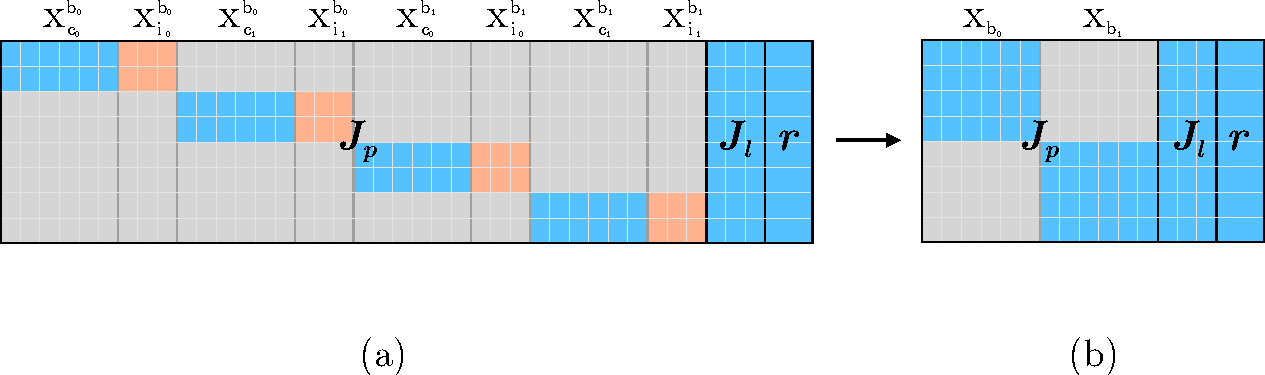
\includegraphics[width=\linewidth]{images/rootba-mod.pdf}
    \caption{Estructura de un Landmark Block. (a)~RootBA original: estado por cámara de dimensión $d_p = 9$, incluyendo parámetros intrínsecos $x_i$ en naranja. (b)~Versión adaptada: $d_p = 6$ (intrínsecos eliminados), con observaciones de múltiples cámaras del rig acumuladas en la variable de body $x_b$.}
    \label{fig:landmark_block}
\end{figure}


\section{Experimentos}
\label{sec:experiments}
\begin{figure*}[!htbp]
    \centering
    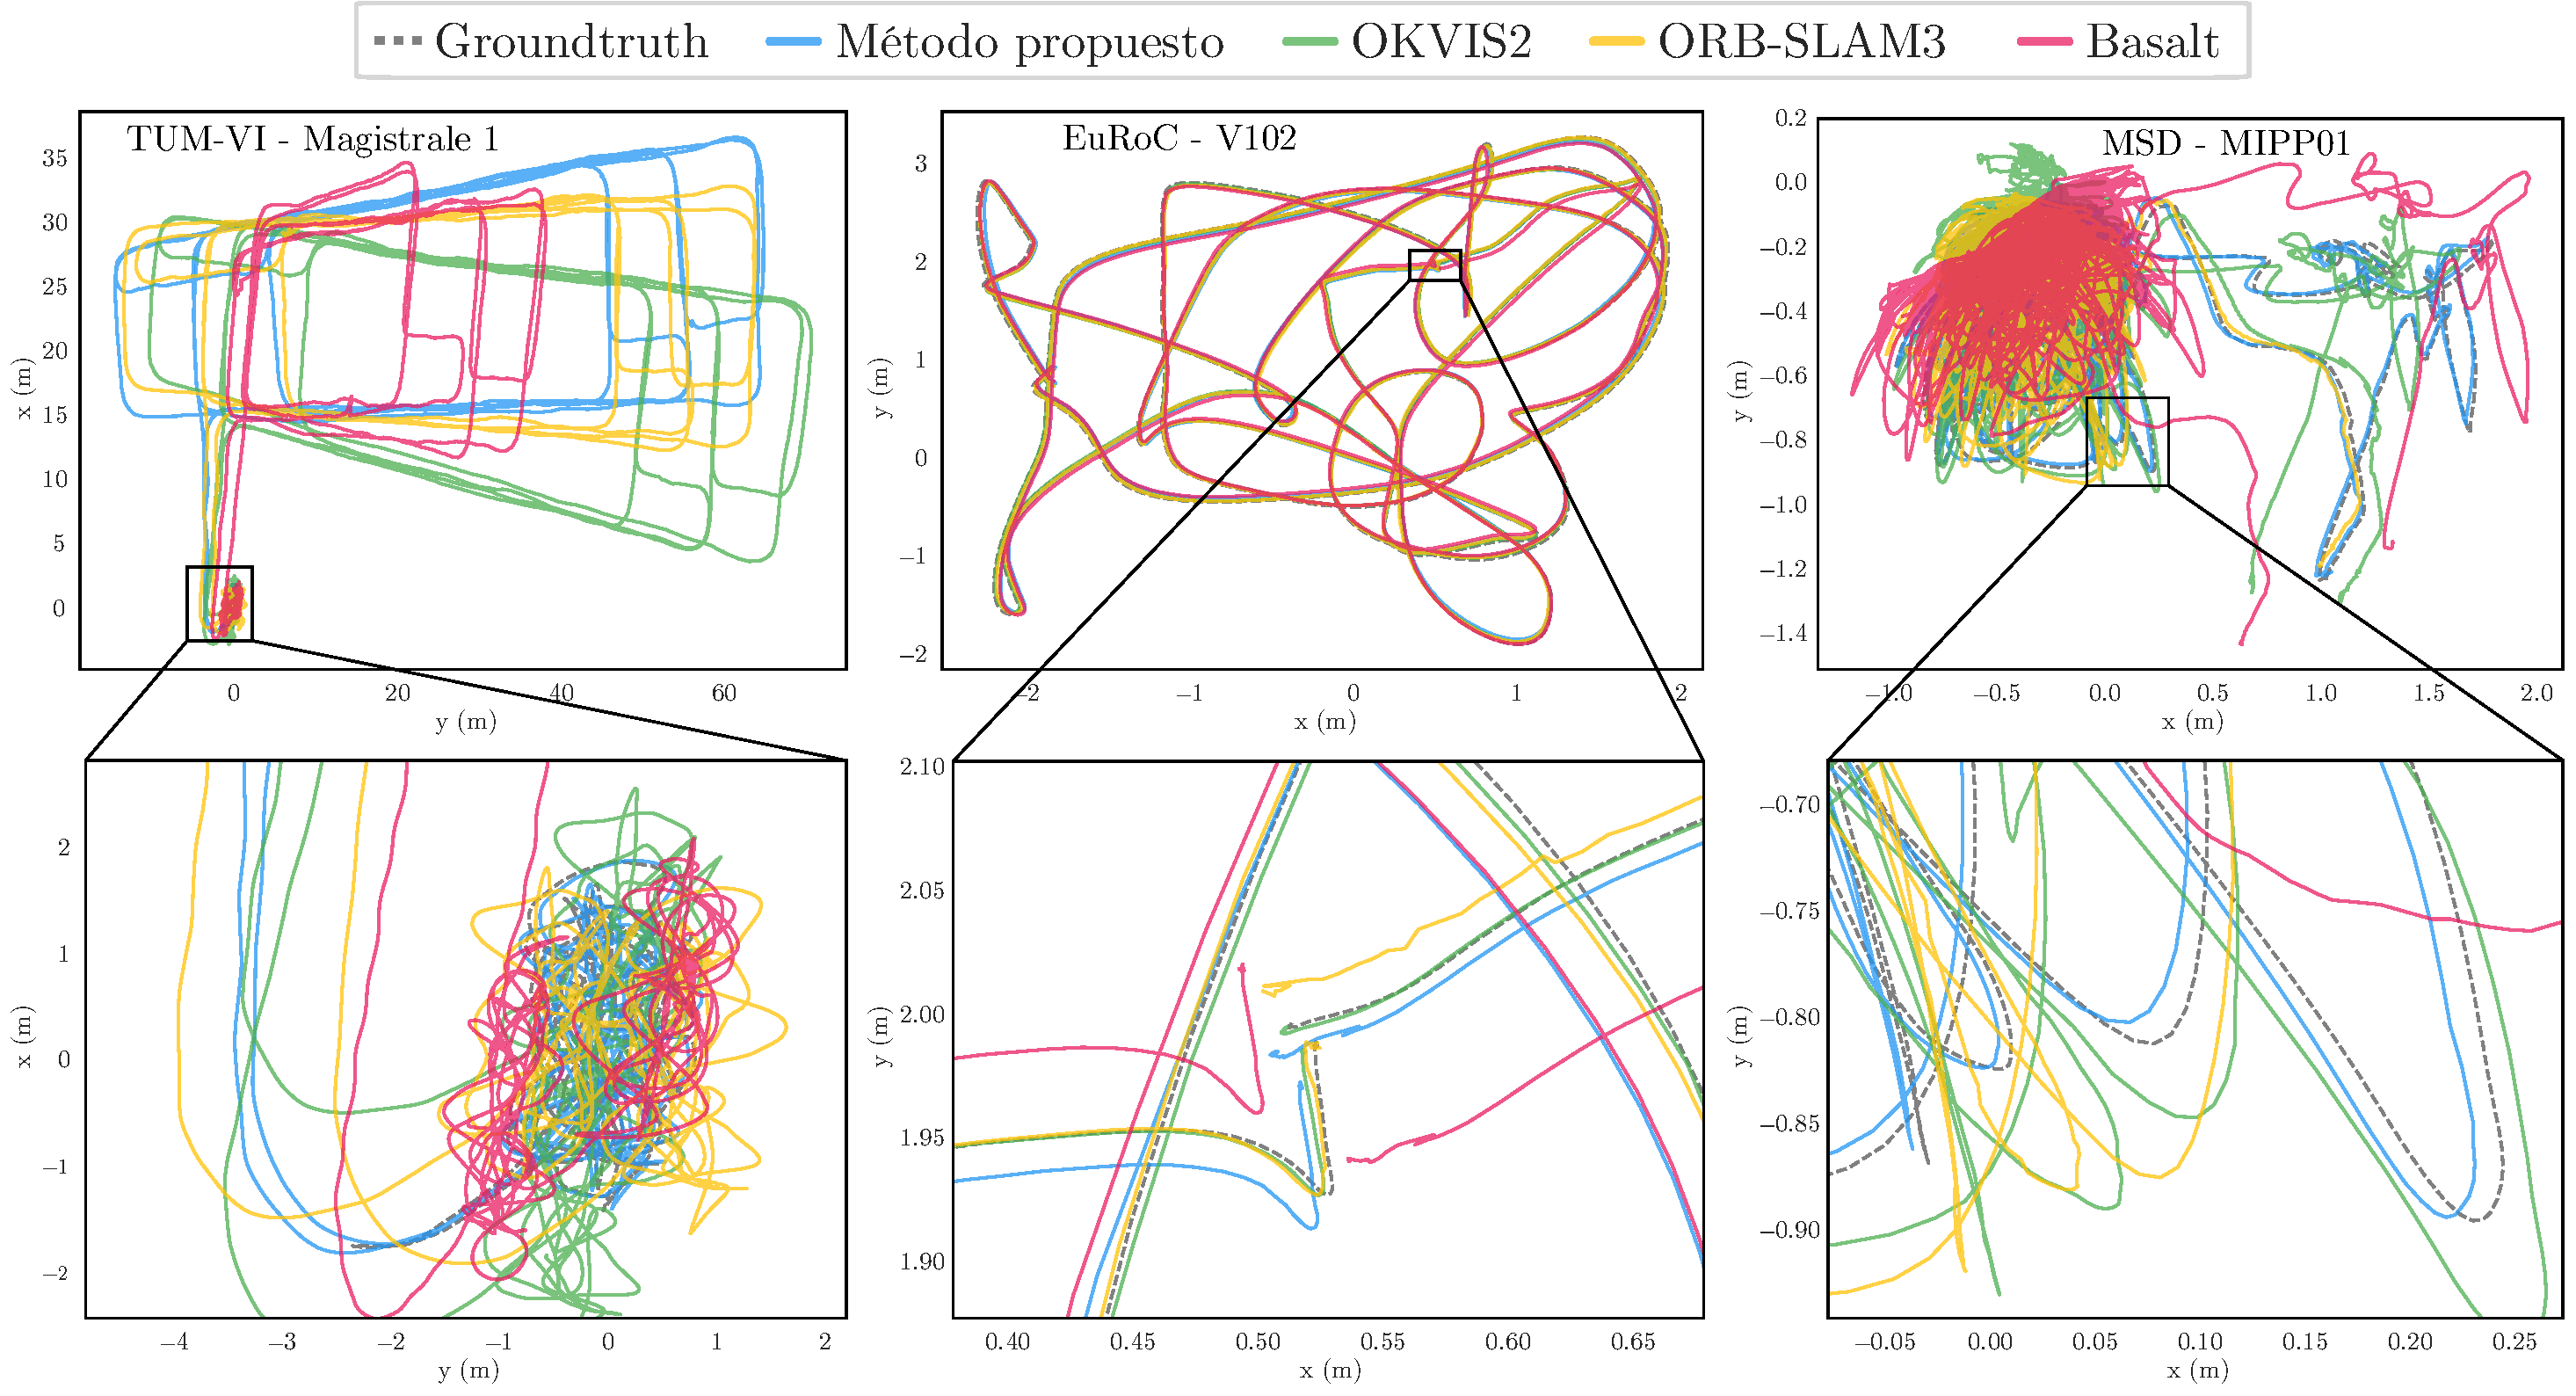
\includegraphics[width=1\linewidth]{images/trajectories.pdf}
    \caption{Ejemplos de trayectorias para secuencias de distintos datasets, con ampliaciones en partes que resultan de interés. Se comparan Basalt en su versión VIO, con el sistema propuesto, y OKVIS2 y ORB-SLAM3 como referencias del estado del arte de VI-SLAM. En Magistrale 1 el sistema propuesto fue el único capaz de detectar el ciclo al reingresar en la habitación. Como se observa en la ampliación de su trayectoria, esta secuencia solo cuenta con ground-truth en la parte de la habitación, al comienzo y al final. En V102, si bien el método propuesto mejora la estimación del VIO de Basalt, no alcanza la precisión de OKVIS2 y ORB-SLAM3. Por último, en MIPP01, el método propuesto es el único capaz de mantener el drift acotado durante toda la secuencia. Tanto OKVIS2 como Basalt acumulan drift considerable, evidenciado por la gran separación entre el inicio y el fin de sus trayectorias. ORB-SLAM3 no es capaz de mantener el tracking y consigue estimar solo el 85\% del total de la secuencia.}
    \label{fig:trajectories}
\end{figure*}

Presentamos experimentos para mostrar las capacidades del sistema y apoyar nuestras afirmaciones.
Se evaluó el método propuesto frente a OKVIS2 y ORB-SLAM3, ambos ejecutados en su modo VI-SLAM
estéreo con cierre de ciclos y optimización final de bundle adjustment, sobre tres datasets públicos: EuRoC~\cite{burri2016euroc} (11 secuencias), TUM-VI~\cite{schubert2018tum} (28 secuencias) y el Monado SLAM Dataset~\cite{demayo2025monadoslamdataset} (MSD,
64 secuencias). En todos los experimentos se evalúa la estimación no causal de la trayectoria.
Los experimentos se realizaron en un procesador Intel Core i5-13600 con 32 GB de RAM, a excepción del experimento de rendimiento contra OKVIS2 y ORB-SLAM3, que fue realizado en un procesador Intel Core Ultra 9 285H con 32 GB de RAM.

\subsection{Métricas de datasets públicos}

La Tabla~\ref{tab:sota_summary} muestra la media del ATE para cada sistema en los tres datasets.

\begin{table}[ht]
\centering
\caption{ATE medio por grupo de secuencias [m].}
\label{tab:sota_summary}
\begin{threeparttable}
\begin{tabular}{l rrr}
\toprule
\textbf{Secuencia}
& \textbf{Método propuesto} & \textbf{OKVIS2} & \textbf{ORB-SLAM3}\tnote{*} \\
\midrule
\multicolumn{4}{l}{\textit{MSD}} \\
MI (Valve Index)      & \textbf{0.05}  & 2.20           & 55.83          \\
MO (Odyssey+)      & \textbf{0.21}  & 0.42           & \textbf{0.21}  \\
MG (HP Reverb G2)      & \textbf{0.04}  & 0.11           & 8.25           \\
\midrule
\multicolumn{4}{l}{\textit{EuRoC}} \\
Machine Hall        & 0.08           & \textbf{0.04}  & 0.05           \\
Vicon Room 1        & 0.07           & \textbf{0.02}  & 0.03           \\
Vicon Room 2        & 0.09           & \textbf{0.02}  & \textbf{0.02}  \\
\midrule
\multicolumn{4}{l}{\textit{TUM-VI}} \\
Corridor   & 0.08           & 0.09           & \textbf{0.06}  \\
Magistrale & 0.85           & \textbf{0.28}  & 0.81           \\
Outdoors   & 62.26          & \textbf{11.60} & 17.87          \\
Room       & \textbf{0.01}  & \textbf{0.01}  & \textbf{0.01}  \\
Slides     & 0.92           & 0.54           & \textbf{0.46}  \\
\bottomrule
\end{tabular}
\begin{tablenotes}
  \footnotesize
  \item[*\!] Promedio de frames procesados y secuencias sin trayectoria:
  80\% - 3, 96\% - 1 y 92\% - 2 para MG, MO y MI respectivamente.
\end{tablenotes}
\end{threeparttable}
\end{table}

En el MSD, el método propuesto es altamente superador. Esto se debe a que los demás sistemas poseen menos robustez y en múltiples secuencias acumulan un error alto o pierden la localización.
ORB-SLAM3 es el menos robusto, ya que no puede completar el procesamiento de la totalidad de frames en múltiples secuencias.

En las secuencias más controladas de TUM-VI, como \textit{Room} y \textit{Corridor}, el método propuesto consigue igualar la precisión de los otros sistemas.

Sin embargo, en las demás secuencias de TUM-VI y EuRoC, OKVIS2 y ORB-SLAM3 obtienen los mejores resultados. La diferencia es especialmente notable en \textit{Outdoors}, donde la escasez de oportunidades de cierre de ciclos hace que los sistemas operen prácticamente como versiones VIO puras. En este contexto, OKVIS2 se destaca por su capacidad de detectar ciclos incluso cuando la superposición entre dos escenas es baja y ocurre en un intervalo de tiempo breve.
La Figura~\ref{fig:trajectories} muestra ejemplos cualitativos de trayectorias para secuencias representativas de los tres datasets.

\subsection{Rendimiento del sistema propuesto}

La Figura~\ref{fig:mgo04_frame_timings} muestra el tiempo de procesamiento por frame
del método propuesto para la secuencia MGO04 del Monado SLAM Dataset.
El promedio móvil se mantiene por debajo
del límite de tiempo real, lo que confirma la viabilidad del sistema
propuesto para aplicaciones como VR/AR. En contraste, OKVIS2 supera el límite en gran medida,
y ORB-SLAM3 lo supera levemente, pese a procesar solo dos de las cuatro cámaras. En este experimento no se contemplaron los tiempos de ejecución de las optimizaciones globales que los sistemas ejecutan offline.

\begin{figure}[!htbp]
    \centering
    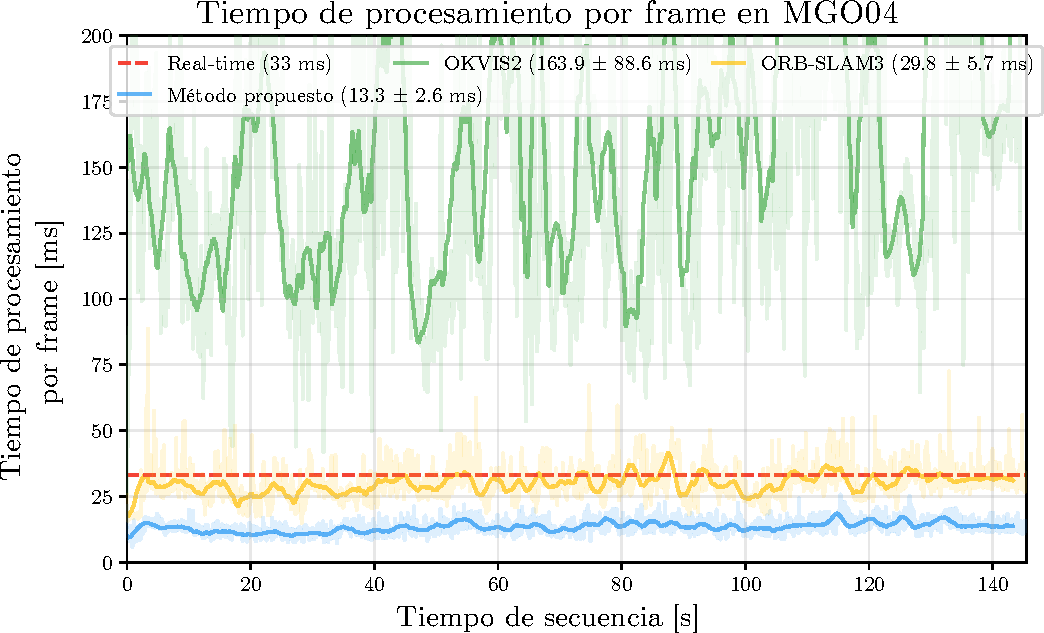
\includegraphics[width=1\linewidth]{images/MGO04.timings.sp.pdf}
    \caption{Tiempo de procesamiento por frame para cada sistema en la secuencia MGO04 del MSD, que cuenta con cuatro cámaras, en un procesador Intel Core Ultra 9 285H con 32 GB de RAM. Se muestra un promedio móvil con una ventana de 2 segundos (60 frames). En el fondo, los datos sin procesar muestran outliers y jitter para cada sistema. Una línea roja marca el límite de tiempo para la operación en tiempo real. Notar que ORB-SLAM3 procesa solo dos de las cuatro cámaras disponibles.}
    \label{fig:mgo04_frame_timings}
\end{figure}

La Figura~\ref{fig:msd_rootba_times} muestra los tiempos de ejecución de la optimización
global con la adaptación de RootBA en precisión simple y doble para los mapas globales de las secuencias del MSD. La precisión simple reduce la mediana del tiempo de optimización en un 50\% en MSD y EuRoC, y en un
42\% en TUM-VI, sin degradar la precisión de la estimación de trayectoria.

\begin{figure}[!htbp]
    \centering
    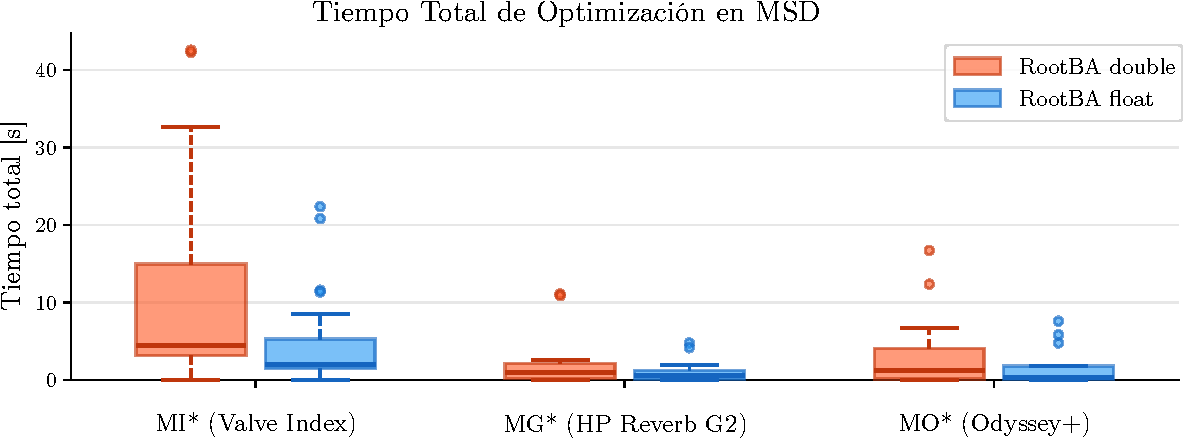
\includegraphics[width=1\linewidth]{images/msd.rootba.times.sp.pdf}
    \caption{Boxplots de tiempos totales de ejecución de la adaptación de RootBA en precisión simple y doble para cada tipo de secuencia del MSD. Ambas versiones fueron ejecutadas sobre el mismo mapa.}
    \label{fig:msd_rootba_times}
\end{figure}


\section{Conclusiones y trabajo futuro}
\label{sec:conclusions}
En este trabajo presentamos un sistema VI-SLAM robusto, preciso y de tiempo real, construido sobre Basalt y BasaltXR. Nuestras contribuciones principales son la extensión de Basalt con un mapa persistente para asociación de datos a largo plazo, y una técnica de bundle adjustment que optimiza el mapa global de forma eficiente.

Los resultados experimentales validan estas afirmaciones. El sistema mantiene la operación en tiempo real de Basalt incluso tras convertirlo en un sistema VI-SLAM completo, gracias a una arquitectura asíncrona que aísla las operaciones costosas del mapa del resto del pipeline. Comparado con sistemas VI-SLAM de bajos requisitos computacionales, es el más eficiente. En cuanto a precisión, es comparable con el estado del arte, con especial fortaleza en entornos cerrados, típicos de VR/AR. Finalmente, la técnica de bundle adjustment propuesta es numéricamente estable, lo que permite operar en precisión simple con una mejora sustancial de rendimiento.

Como trabajo futuro se proponen las siguientes líneas: integrar la optimización de bundle adjustment en el mapa persistente para que se ejecute de manera frecuente y online; incorporar términos de la IMU en la optimización global; mejorar la eficiencia y robustez de la asociación de datos a mediano plazo, en particular mediante la reintroducción de keyframes a la ventana del back-end; y fortalecer las verificaciones de consistencia en la detección de ciclos, para habilitarlas en entornos más desafiantes y con un menor número de correspondencias.

% también mejorar el culling
% mejorar la calidad del mapa


%\section{Apéndice}
%\label{sec:appendix}
%\input{src/appendix.tex}

%\section*{Agradecimientos}
%Este trabajo fue apoyado por la Universidad Nacional de Rosario (PCCT-UNR 80020220600072UR).


\bibliographystyle{IEEEtran}
\bibliography{biblio}

\end{document}


